
This chapter describes the estimation achieved through COCOMO II: a complex, non linear model that takes in account the characteristics of the product, people and processes.
In order to generate the Constructive Cost Model we decided to use an online COCOMO II calculator on \url{http://csse.usc.edu/tools/COCOMOII.php}, using the  FP Sizing Method.
We also usedCOCOMO II - Model Definition Manual to make better choices of the parameters we had to insert into the  model.
\begin{itemize}
  \itemBold{Software Size}
    \begin{itemize}
      \itemBold{Unadjusted Function Points} The value FP has been taken as parameter, so 149 is the value chosen for this field.
      \itemBold{Language} The language of choice is Java, and not only Java EE, because the software is possibly a combination of different flavours of Java  (Java  SE, Java  EE and Java  for Android).
    \end{itemize}
  \itemBold{Software Scale Drivers}
    \begin{itemize}
      \itemBold{Precedentedness} Since we had a previous experience using Java SE for medium-size projects, but we have never used Java EE for developing such a big application we  decided to set this parameter to Nominal.
      \itemBold{Development Flexibility} Given that we had not strict specifications so we set this parameter to High.
      \itemBold{Architecture/Risk Resolution} Since we have designed several documents before the actual development, including this PPD, the development of the system to be has little chances of failing, so we choose  a  Nominal value.
      \itemBold{Team Cohesion} After a few days dedicated to create a efficient and fast workspace, the cohesion reached a Very High  level.
      \itemBold{Process Maturity} We understood, support and follow the process so we choose a High level for this parameter.
    \end{itemize}
  \itemBold{Software Cost Drivers}
    \begin{itemize}
      \item Product
        \begin{itemize}
          \item Required Software Reliability: Given that a failure in the software system could lead to moderate problems we choose Nominal level.
          \item Data Base Size:  Since we have a distributed application, the focus is on the lines of code instead of being on the size of the testing Database; so we choose a Low level parameter.
          \item Product Complexity: We made an average of the various complexity areas and we choose a High level parameter.
          \item Developed for Reusability:  We decided to develop reusable system components, so we came up with an High level parameter.
          \item Documentation Match to Lifecycle Needs: The standard level of documentation is required, so the chosen level is Nominal.
        \end{itemize}
      \item Personnel
        \begin{itemize}
          \item Analyst Capability: The personnel demonstrated a Nominal level of analysis ability.
          \item Programmer Capability: The personnel demonstrated efficiency working together as a team, so we chose High level for this  parameter.
          \item Personnel Continuity: The project will be developed always by the initial programmers, so the project’s annual personnel turnover is very low (7 % for year). For this reason we have chosen High for this parameter.
          \item Application Experience: Since the last time the development team has worked on a so complicated project was a year ago, we have chosen Nominal for this parameter.
          \item Platform Experience: The same as Application Experience ; we have chosen Nominal level for this parameter too.
          \item Language and Toolset Experience: The team is quite familiar with the development, analysis and design representation, so we choose High level for this parameter.
        \end{itemize}
      \item Platform
        \begin{itemize}
          \item Time Constraint: We have no relevant time constraints, so we choose Nominal level for this parameter.
          \item Storage Constraint: We have no relevant storage constraint, so we choose Nominal level for this parameter.
          \item Platform Volatility: Our hardware and software platforms will not change often, so we will have  no volatility and therefore we choose a Low level for this  constraint.
        \end{itemize}
      \item Project
        \begin{itemize}
          \item Use of Software Tools: The team is provided of a set of strong and mature life-cycle tools, moderately integrated one into each other.  So we choose an High level for this  parameter.
          \item Multisite Development: The team is in average fully collo- cated, so the chosen level is Nominal.
          \item Required Development Schedule: The project is not sub- jected on a particular constraint oppression, so we have chosen Nominal for this parameter.
        \end{itemize}
      \end{itemize}
    \itemBold{Maintenance} This value is set to Off
    \itemBold{Software Labour Rates}
      \begin{itemize}
        \item Cost per Person-Month (Dollars): We have chosen the average value of 1500\$/month for this parameter.
      \end{itemize}
    \end{itemize}


  \begin{center}
  	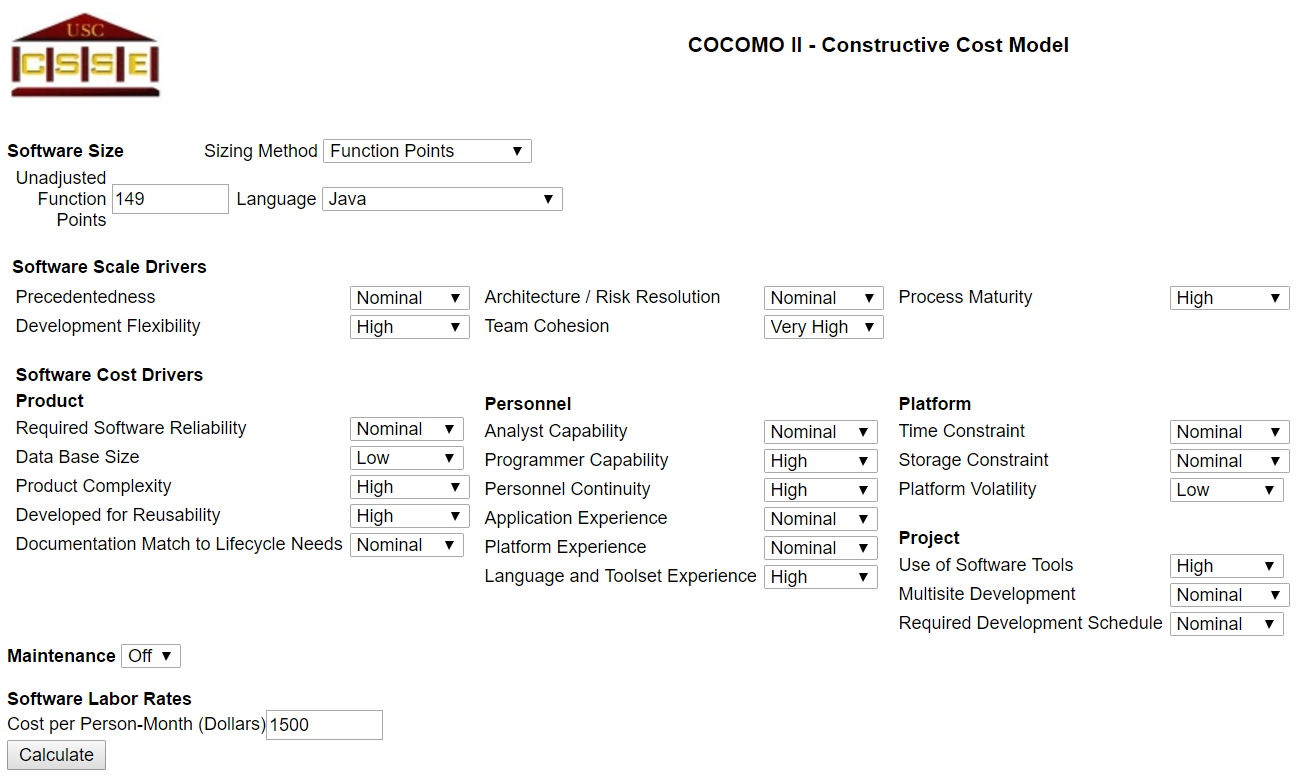
\includegraphics[width=\textwidth]{Resources/Cocomo_2.PNG}
    \captionof{figure}{COCOMO Parameters}
  	\label{COCOMO tools}
  \end{center}
  \newpage{}
  And here below we can see the result:

  \begin{center}
  	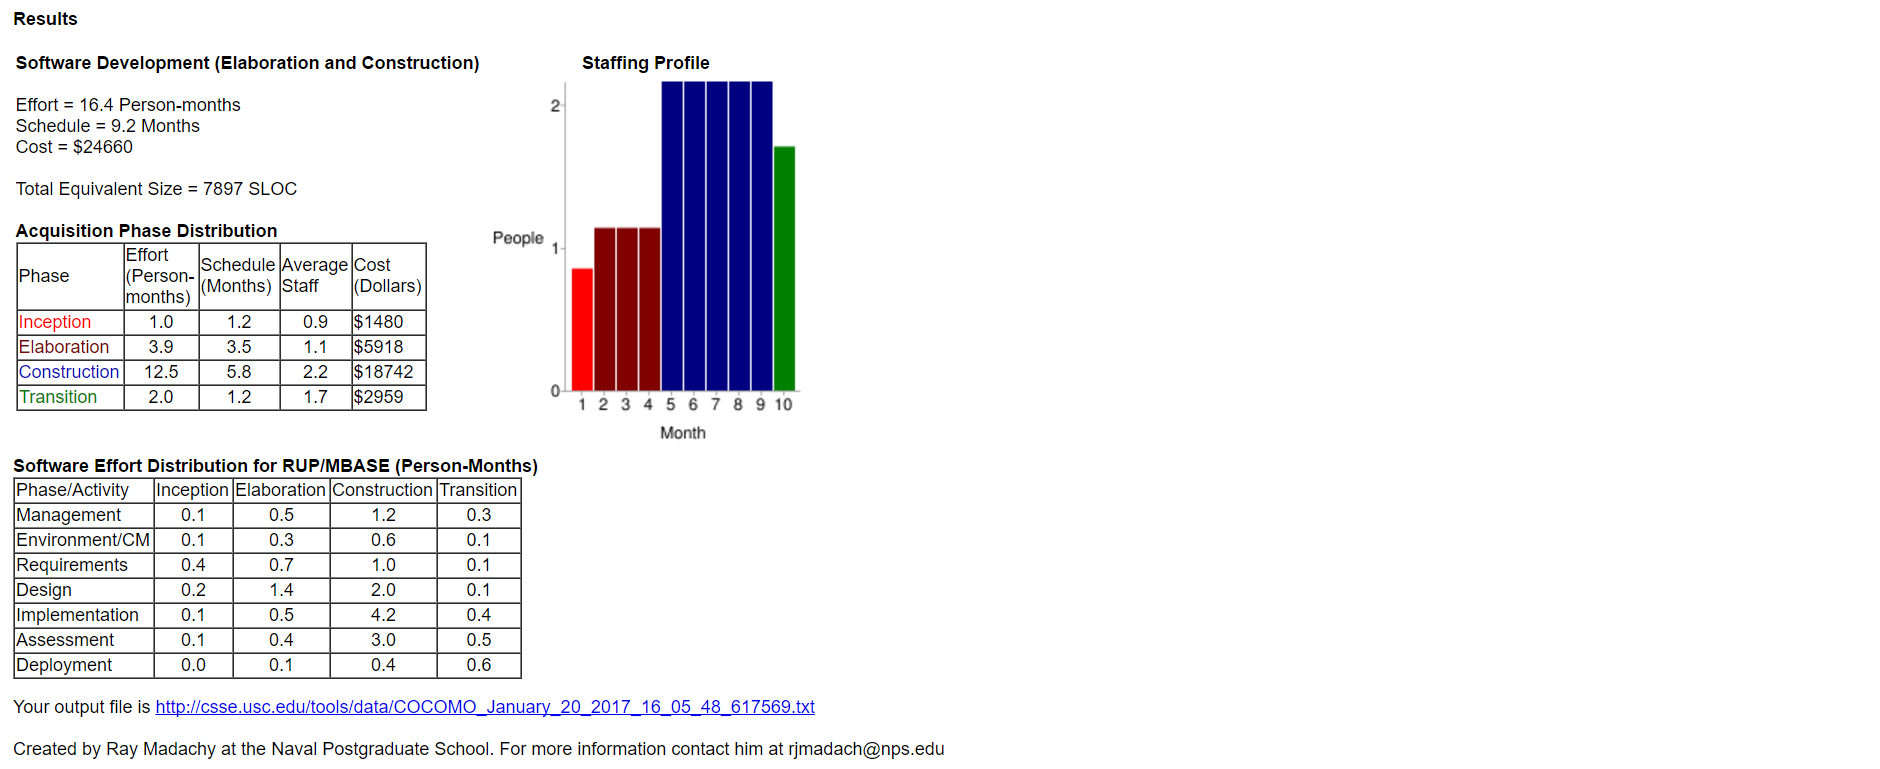
\includegraphics[width=\textwidth]{Resources/Cocomo_1.PNG}
    \captionof{figure}{COCOMO Results}
  	\label{COCOMO result}
  \end{center}
